\section{Auswertung}
\label{sec:Auswertung}
\FloatBarrier
\subsection{Bestimmung der mittleren freien Weglänge und des Kontaktpotentials}
%\begin{figure}
%  \centering
%  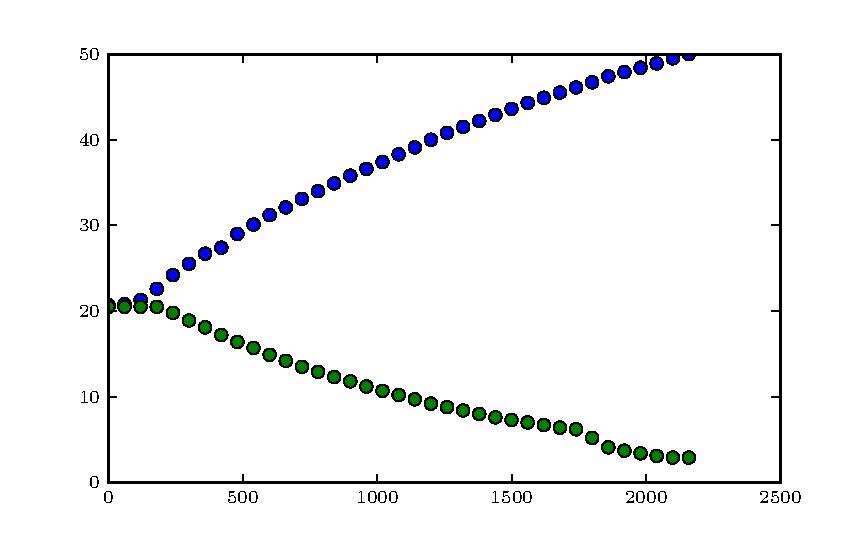
\includegraphics{plot.pdf}
%  \caption{Plot.}
%  \label{fig:plot}
%\end{figure}
\subsubsection{Bestimmung der mittleren freien Weglänge}
Die mittlere freie Weglänge ergibt sich mit Formel \eqref{eqn:freiewegl} zu
\begin{equation*}
	\bar{w} = 1
\end{equation*}

\FloatBarrier
\subsection{Bestimmung der Skalierungen}
Die abgelesenen Werte für die Skalierung der Messung bei $\SI{150}{\celsius}$ sind in
Tabelle \ref{tab:skalierung_a_2} aufgetragen.
\begin{table}
	\centering
	\caption{Messdaten zur Bestimmung der Grenzspannung $U_\mathrm{G}$.}
	\label{tab:ug}
	\begin{tabular}{cc}
		\toprule
		$U_{\mathrm{B}}$ / $\si{\volt}$ & Abstand / $\si{\centi\meter}$ \\
		\midrule
		0 & 0 \\
		1 & 2.1 \\
		2 & 4.1 \\
		3 & 5.9 \\
		4 & 7.9 \\
		5 & 9.9 \\
		6 & 12.0 \\
		7 & 14.0 \\
		8 & 16.1 \\
		9 & 18.1 \\
		10 & 20.2 \\
		\bottomrule
	\end{tabular}
\end{table}
Zur Skalierung der Messung der integralen Energieverteilung wird zunächst jeder Abstand zwischen zwei Punkten bekannter Bremsspannung gemessen und über alle Abstände mittels python/scipy \cite{scipy} gemittelt.
Die zugehörigen Messdaten finden sich in Tabelle \ref{tab:skalaa}.
Es ergibt sich als mittlere Länge $x$ pro $\SI{1}{\volt}$:
\begin{equation}
	x=\SI{20.3(3)}{\milli\meter\per\volt} \mathrm{,}
\end{equation}
beziehungsweise als mittlere Spannung pro Kästchen auf dem Millimeterpapier:
\begin{equation}
	V_1= \SI{4.93(7)e-02}{\volt\per\milli\meter} \mathrm{.}
\end{equation}
Da die Fehler unter der Messauflösung liegen, werden sie im Folgenden nicht weiter berücksichtigt.

Um aus der integralen Energieverteilung schließlich die differentielle Energieverteilung zu erhalten, wird die Steigung der integralen Energieverteilung mittels Steigungsdreiecken, wie in Abbildung \ref{fig:originaleins} eingezeichnet, bestimmt.


\begin{table}
	\centering
	\caption{Messdaten zur Bestimmung der Achsenskalierung bei $T=\SI{299.75}{\kelvin}$.}
	\label{tab:skalaa}
	\begin{tabular}{cc}
		\toprule
		Bereich $U_{\mathrm{A}}$ / $\si{\volt}$ & Abstand zwischen Messpunkten/ $\si{\milli\meter}$ \\
		\midrule
		0-1 & 21.5 \\
		1-2 & 18.5 \\
		2-3 & 20.0 \\
		3-4 & 20.0 \\
		4-5 & 20.0 \\
		5-6 & 19.5 \\
		6-7 & 20.5 \\
		7-8 & 20.5 \\
		8-9 & 20.5 \\
		9-10 & 22.0 \\
		\bottomrule
	\end{tabular}
\end{table}
%%%%%%%%%%%%%%%%%%%%%%%%%%%%%%%%%%%%%%%%%%%%%%%%%%%%%%%%%%%%%%
\FloatBarrier
\subsection{Franck-Hertz-Kurve}
Zunächst wird erneut die Skalierung der x-Achse bestimmt.
Die gemessenen Abstände finden sich in Tabelle \ref{tab:franckie}.
\begin{table}
 \centering
 \caption{Messdaten zur Bestimmung der Achsenskalierung der Franck-Hertz-Kurve.}
 \label{tab:franckie}
 \begin{tabular}{cc}
	 \toprule
	 Bereich $U_{\mathrm{B}}$ / $\si{\volt}$ & Abstand zwischen Messpunkten/ $\si{\milli\meter}$ \\
	 \midrule
	 0-5 & 16.5 \\
	 5-10 & 18.0 \\
	 10-15 & 17.5 \\
	 15-20 & 17.5 \\
	 20-25 & 18.5 \\
	 25-30 & 17.5 \\
	 30-35 & 17.0 \\
	 35-40 & 19.0 \\
	 40-45 & 18.5 \\
	 45-50 & 18.5 \\
	 50-55 & 18.0 \\
	 \bottomrule
 \end{tabular}
\end{table}
Es ergibt sich als mittlere Länge $x$ pro $\SI{5}{\volt}$:
\begin{equation}
	x=\SI{17.9(2)}{\milli\meter\per\volt} \mathrm{,}
\end{equation}
beziehungsweise als mittlere Spannung pro Kästchen auf dem Millimeterpapier:
\begin{equation}
	V_1= \SI{28.0(3)e-02}{\volt\per\milli\meter} \mathrm{.}
\end{equation}
Da die Fehler unter der Messauflösung liegen, werden sie im Folgenden erneut nicht weiter berücksichtigt.
Es wird nun der Abstand zwischen den Maxima der Franck-Hertz-Kurve gemessen. Diese Abstände entsprechen hierbei, multipliziert mit der Elementarladung $\symup{e}_0$ der 1. Anregungsenergie des Hg-Atoms (vgl. Formel \eqref{eqn:photonemission}).
In Tabelle \ref{tab:hertzchen} finden sich die gemessenen Abstände sowie die daraus bestimmten $U_\mathrm{1}$.
\begin{table}
	\centering
	\caption{Abständer der Maxima der Franck-Hertz-Kurve.}
	\label{tab:hertzchen}
	\begin{tabular}{ccc}
		\toprule
		k& Abstand $U_{\mathrm{k+1}}-U_{\mathrm{k}}$ / $\si{\milli\meter}$ & $\Delta E=E_1 - E_0$/ $\si{\electronvolt}$ \\
		\midrule
3&17.5 & 4.9\\
4&18.0 & 5.0\\
5&18.5 & 5.2\\
6&17.5 & 4.9\\
7&19.5 & 5.5\\
8&20.0 & 5.6\\
9&19.0 & 5.3\\
11&21.0 & 5.9\\
\end{tabular}
\end{table}

Aus einer Mittelung mittels python/scipy \cite{scipy} ergibt sich
\begin{equation}
	\Delta E=\SI{5.3(1)}{\electronvolt} \mathrm{.}
\end{equation}
Mit der Beziehung $\lambda=\frac{c}{\nu}$ und unter Verwendung von Formel
\eqref{eqn:photonemission} ergibt sich für die Wellenlänge des emmitierten Lichts
\begin{equation}
	\lambda=\SI{235(5)}{\nano\meter}
\end{equation}
Da für den Glühdraht und für die Beschleunigungselektrode ein Material mit unterschiedlicher Elektronenaustrittsarbeit verwendet wurde, ist die Franck-Hertz-kurve um das Kontaktpotential verschoben.
Die ersten Maxima können aus der aufgenommenen Franck-Hertz-Kurve allerdings nicht eindeutig bestimmt werden, daher wird ihre Lage anhand der bekannten
%%%%%%%%%%%%%%%%%%%%%%%%%%%%%%%%%%%%%%%%%%%%%%%%%%%%%%%%%%%%%%%%%%%%%%%%%%%%%%%%%%%%%%%%%%%%
\FloatBarrier
\subsection{Bestimmung der Ionisationsspannung von Quecksilber}
In Abbildung \ref{fig:ionisation} ist der Auffängerstrom $I_{\mathrm{A}}$ in Abhängigkeit
von der Beschleunigungsspannung $U_{\mathrm{B}}$ bei einer Gegenspannung von $-\SI{30}{\volt}$
aufgetragen.
